\documentclass[11pt,a4paper]{article}
\usepackage[margin=24mm,headheight=15pt]{geometry}
\usepackage{fontspec}
\setmainfont{Latin Modern Roman}
\setsansfont{Latin Modern Sans}
\setmonofont[Scale=0.88]{Latin Modern Mono}
\usepackage{microtype,graphicx,booktabs,longtable,tabularx,array}
\usepackage[table]{xcolor}
\usepackage{amsmath,tikz,listings,enumitem,fancyhdr}
\usetikzlibrary{arrows.meta,positioning}
\usepackage[numbers,sort&compress]{natbib}
\usepackage[hyphens]{url}
\usepackage[colorlinks=true,linkcolor=black,citecolor=black,urlcolor=black]{hyperref}
\hypersetup{pdftitle={TPC-DS on MariaDB: Implementation and Experimental Evaluation},pdfauthor={INFO-H-419 project group}}
\definecolor{papergray}{HTML}{F3F3F3}
\pagestyle{fancy}
\fancyhf{}
\fancyhead[L]{\small TPC-DS on MariaDB}
\fancyhead[R]{\small INFO-H-419}
\fancyfoot[C]{\thepage}
\renewcommand{\headrulewidth}{0.3pt}
\setlength{\parindent}{0pt}
\setlength{\parskip}{0.5em}
\setlength{\emergencystretch}{3em}
\setlist{itemsep=2pt,topsep=3pt}
\renewcommand{\arraystretch}{1.15}
\newcolumntype{Y}{>{\raggedright\arraybackslash}X}
\DeclareRobustCommand{\file}[1]{\path{#1}}
\lstset{basicstyle=\ttfamily\footnotesize,breaklines=true,columns=fullflexible,
  keepspaces=true,showstringspaces=false,backgroundcolor=\color{papergray},
  keywordstyle=\color{black},commentstyle=\color{gray},frame=single,
  rulecolor=\color{black!15},xleftmargin=4pt,xrightmargin=4pt,
  aboveskip=7pt,belowskip=7pt}
% Edit these placeholders before submission. No student identity is inferred.
\newcommand{\GroupNumber}{[Group number]}
\newcommand{\GroupMembers}{%
  \textit{[Full name 1]} & \textit{[Student ID 1]} \\
  \textit{[Full name 2]} & \textit{[Student ID 2]} \\
  \textit{[Full name 3]} & \textit{[Student ID 3]} \\
  \textit{[Full name 4]} & \textit{[Student ID 4]} \\
}
\newcommand{\CourseLecturer}{[Lecturer name]}

\input{generated/metrics}

\begin{document}
\begin{titlepage}
\centering
{\Large UNIVERSITÉ LIBRE DE BRUXELLES\par}
\vspace{4mm}
{\large Erasmus Mundus Joint Master in\par Data Engineering and Artificial Intelligence\par}
\vspace{25mm}
{\Huge\bfseries TPC-DS on MariaDB\par}
\vspace{8mm}
{\Large Implementation and Experimental Evaluation\par}
\vspace{16mm}
{\large INFO-H-419 --- Data Warehouses\par Part I project report\par}
\vspace{15mm}
{\large\GroupNumber\par}
\vspace{5mm}
\begin{tabular}{ll}\toprule Group members & Student IDs \\ \midrule
\GroupMembers
\bottomrule\end{tabular}
\vspace{8mm}
\par Course lecturer: \CourseLecturer
\vfill
October 2026
\end{titlepage}

\pagenumbering{roman}
\section*{Abstract}
This project implements and evaluates TPC-DS analytical queries on MariaDB.
The implementation combines the official v4.0.0 data generator, a relational
retail warehouse, MariaDB SQL adaptations and a Docker execution workflow.
All 99 query identifiers are supported, with \AdoptedCount{} adopted query
optimization variants integrated into the complete workload.

The evaluation includes complete original and adopted workloads at scale
factors \MeasuredScales{}, using a 2~GiB InnoDB buffer pool. The eight passes
execute \TotalQueryExecutions{} query files. At SF4, the original workload
completed in \SFfourOriginalSeconds{} seconds and the adopted workload in
\SFfourAdoptedSeconds{} seconds. Result comparison confirms matching values
for all 99 queries at each scale. Recorded runtime reductions range from
\MinRuntimeReduction\% to \MaxRuntimeReduction\% across the four sizes.
Repeated local SF1 experiments complement these measurements
with per-query medians, execution plans and targeted semantic tests.

The report presents the implementation pipeline, result-validation procedure,
physical-design experiments and representative SQL transformations. These
include predicate pushdown, conditional aggregation, late dimension joins and
window-query restructuring. The results illustrate how analytical query
structure, access paths and memory settings affect execution time. The source
package preserves the executed SQL, answers, timing records and replication
commands used to produce the reported measurements.

\tableofcontents
\clearpage
\pagenumbering{arabic}

\section{Introduction}
Data warehouses organize historical business data for analytical processing.
Their workloads typically join large fact tables with descriptive dimensions
and aggregate measures over substantial portions of the database. Query
performance therefore depends on the interaction between logical SQL,
physical design, optimizer decisions and the available memory budget.

The INFO-H-419 project applies these concepts through an implementation of
TPC-DS. Our objectives are to execute the benchmark's analytical workload on
MariaDB, validate the results of the SQL adaptations, study optimization
techniques, and measure execution time at different dataset sizes.

\subsection{Starting point and project contributions}
The implementation builds on the \file{mariadb-tpcds} repository
\citep{repository}, including its toolkit integration, schema, loader, adapted
query instances and earlier experiments. The project also draws on
\file{tpcds-run-tool} \citep{referenceimplementation}. These resources provided
an operational starting point for the subsequent engineering and evaluation.

The completed work comprises SQL optimization variants, controlled local
experiments, NULL-safe rollup translations, full answer capture, complete
99-query Docker execution, configurable memory settings, explicit data seeds
and preservation of execution artifacts. The contributed query directories
and source headers record the authorship and selected versions.

This report follows the technology--implementation--evaluation structure used
in earlier course reports on Oracle and PostgreSQL
\citep{oracleexample,postgresexample}. Its measurements come from the MariaDB
execution artifacts described below.

\subsection{Benchmark scope}
TPC-DS models the analytical workload of a retail supplier through its data
model and query templates \citep{tpcds}. The implementation uses these data and
queries for a course experiment. Its execution procedure runs complete query
files serially and reports elapsed time in seconds, together with per-query
answer comparisons and the corresponding database settings.

\section{Technology and warehouse implementation}
\label{sec:implementation}
\subsection{MariaDB and InnoDB}
MariaDB provides the relational query engine and InnoDB supplies the table
storage. The workload exercises joins, exact decimal arithmetic, grouped
aggregation, common table expressions (CTEs), rollups and window functions.
Docker packages the database and toolchain, while Python manages execution,
timing, result serialization and analysis.

The complete Docker workloads use MariaDB 13.0.2. The initial local development
experiments use MariaDB 10.11.14. Their results are presented as separate series.
InnoDB's buffer pool caches database pages \citep{bufferpool}; temporary tables,
join buffers and sort buffers provide additional workspace for query execution.
The Docker measurements use a 2~GiB buffer pool, 32~KiB pages and a persistent
statistics sample setting of 160.

\subsection{Retail model and schema}
\file{sql/01_schema.sql} defines 25 tables, 429 columns and 24 primary keys.
Seven fact tables represent sales, returns and inventory. Seventeen shared
dimensions describe products, customers, dates, locations and related business
attributes; the remaining table records generator metadata.

\begin{table}[htbp]\centering\small
\begin{tabularx}{\linewidth}{lYY}\toprule
Process & Fact tables & Example dimensions \\ \midrule
Store & \file{store_sales}, \file{store_returns} & date, time, customer, item, store \\
Catalog & \file{catalog_sales}, \file{catalog_returns} & date, item, customer, call center, shipping \\
Web & \file{web_sales}, \file{web_returns} & date, item, customer, web site/page \\
Inventory & \file{inventory} & date, item, warehouse \\
\bottomrule\end{tabularx}
\caption{Business processes represented in the implemented warehouse.}
\end{table}

Sales facts have transaction-line grains. Inventory is identified by date,
item and warehouse. Shared dimensions connect the three channels, producing a
constellation of related star and snowflake structures. The schema uses
\file{DECIMAL} measures, \file{DATE} columns, UTF-8 text and explicit collations.

The schema reconciliation in \file{report/04-reconcile-discrepancies.md}
resolves differences between toolkit files and the specification, including
the customer's last-review date key and the spelling of the store tax column.
\file{sql/02_foreign_keys.sql} describes 107 relationships. The saved local SF1
integrity check evaluated all 107 and returned zero orphan rows.

\subsection{Data generation and loading}
The bundled v4.0.0 \file{dsdgen} generates pipe-delimited data with an explicit
scale and \file{RNGSEED=10}. The loader in \file{sql/04_load_data.sql} consumes
the trailing delimiters and converts nullable fields using \file{NULLIF}.
This preserves the generator's representation of NULL values
\citep[Clause~3.4.5]{tpcds}.

Named Docker volumes retain generated files and the loaded database. Generation
markers identify reusable datasets; later runs against the same volume reuse
the loaded warehouse. Schema creation, data loading, index construction and
statistics refresh precede query execution.

\begin{figure}[htbp]\centering
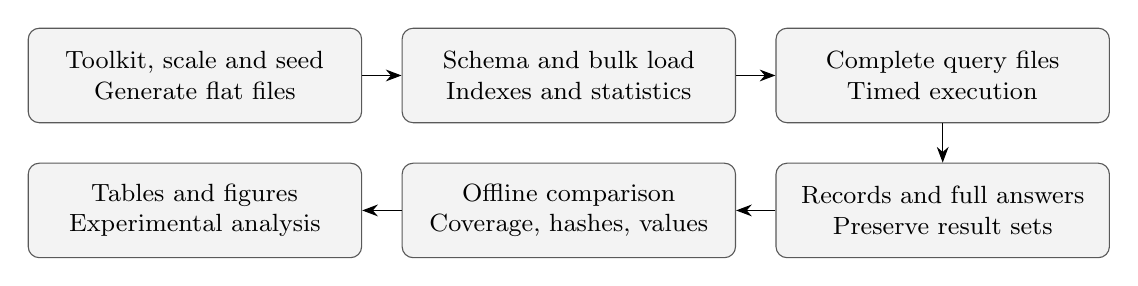
\begin{tikzpicture}[node distance=5mm and 5mm,
 box/.style={draw=black!65,fill=papergray,rounded corners,align=center,
 text width=40mm,minimum height=12mm,font=\small},
 >={Stealth[length=2mm]}]
\node[box] (gen) {Toolkit, scale and seed\\Generate flat files};
\node[box,right=of gen] (load) {Schema and bulk load\\Indexes and statistics};
\node[box,right=of load] (run) {Complete query files\\Timed execution};
\node[box,below=of run] (answers) {Records and full answers\\Preserve result sets};
\node[box,left=of answers] (check) {Offline comparison\\Coverage, hashes, values};
\node[box,left=of check] (report) {Tables and figures\\Experimental analysis};
\draw[->] (gen)--(load);\draw[->] (load)--(run);\draw[->] (run)--(answers);
\draw[->] (answers)--(check);\draw[->] (check)--(report);
\end{tikzpicture}
\caption{The implemented generation, execution and analysis workflow.}
\end{figure}

\subsection{Query preparation and MariaDB adaptation}
\file{queries/mariadb/} contains the 99 adapted originals. The preparation layer
handles date intervals, derived-table aliases, MariaDB rollup syntax and
full-outer-join emulation. Full joins are expressed through a left-join branch
and an unmatched right-join branch combined with \file{UNION ALL}, preserving
duplicate rows.

The execution session enables \file{IGNORE_SPACE} and \file{PIPES_AS_CONCAT}.
The latter preserves concatenated identifiers in queries such as Q5. Each
complete file runs in one connection, retaining its session settings and
variables across statements. Query literals are stored in the committed SQL;
\file{RNGSEED} controls generation of the warehouse data.

\section{Workloads and experimental methodology}
\label{sec:method}
\subsection{Query coverage and optimization count}
\begin{table}[htbp]\centering\small
\begin{tabularx}{\linewidth}{lYr}\toprule
Selector & Workload & Query IDs \\ \midrule
\file{all} & Complete adapted original workload & 99 \\
\file{all-tuned} & Complete workload with adopted optimization variants & 99 \\
\file{tier45} & Original versions of the selected expensive queries & 40 \\
\file{tuned} & Selected queries using the adopted versions & 40 \\
\bottomrule\end{tabularx}
\caption{Query selection through \file{QUERYSET}.}
\end{table}

The adopted workload integrates \AdoptedCount{} optimization variants among
40 selected query IDs. Five selected queries retain their adapted originals:
Q38, Q58, Q66, Q71 and Q77. The remaining 59 IDs also use adapted original SQL.
Thus the complete workload combines 35 selected optimization variants with
64 adapted originals. Appendix~\ref{app:ids} lists the optimization IDs.

The count is generated from the selected source headers. Multiple development
versions of one query contribute one query ID. Index-only contributions and
compatibility fixes are tracked separately from the adopted SQL variants.

\subsection{Experimental configurations}
\begin{table}[htbp]\centering\footnotesize
\begin{tabularx}{\linewidth}{lYY}\toprule
Series & Database configuration & Measurement procedure \\ \midrule
Local SF1 studies & MariaDB 10.11.14; Ryzen 5 3500U; 6.7~GiB host RAM;
2~GiB pool; 16~KiB pages; 16~MiB temporary-table limits & Three ordinary trials
per selected version and profile; full answers and saved plans \\
Docker workloads & MariaDB 13.0.2; 2~GiB pool; 32~KiB pages; statistics sample
160; seed 10 & One serial pass per original/adopted workload; all 99 query files \\
\bottomrule\end{tabularx}
\caption{The development and complete-workload experiment series.}
\label{tab:environments}
\end{table}

The Docker transcript records eight logical CPUs and approximately 6.7~GiB
capacity. Run summaries retain the buffer-pool size, page size, statistics
sample, workspace settings, index count and workload selection. At SF1, SF2
and SF3, both workloads record 190 total indexes. At SF4, the original records 190 and the
adopted workload 188. The timing ratios in this report compare these recorded
original and adopted configurations.

Executed SQL is identified by SHA-256. The preserved bundles include the exact
query versions, including the Q22 revision used by the SF4 adopted run.
Summary hashes connect the report's numeric tables to their input artifacts.

\subsection{Timing and aggregation}
\file{docker/bench.py} measures wall-clock time around the MariaDB client call.
The interval includes connection/session setup, every statement in the query
file and complete XML result transfer. Parsing, hashing and writing JSON occur
after the timer. Generation, loading, index construction and statistics refresh
are measured separately from query execution. The protocol is recorded as
\file{whole-file-xml-v1}.

For scale $S$, workload $W$ and configuration $C$, the serial workload total is
\begin{equation}
 T(S,W,C)=\sum_{q=1}^{99} t(q,S,W,C).
\end{equation}
The reported original/adopted ratio is
\begin{equation}
 R(S)=\frac{T(S,W_o,C_o)}{T(S,W_a,C_a)}.
\end{equation}
Docker query times are recorded to 0.1 seconds. The local studies retain
unrounded individual times, exclude warm-up/probe executions and report
three-run medians and ranges. Instrumented plan diagnostics are stored as a
separate class of execution.

\section{Correctness checks and result validation}
\label{sec:correctness}
\subsection{Complete answer comparison}
The runner saves each query's complete answers using
\file{result-sets-json-v1}. The representation preserves result-set boundaries,
column order, repeated column names, duplicate rows, NULLs, empty strings and
exact returned numeric text.

Artifact checks verify coverage of IDs 1--99, successful execution status,
answer hashes and recorded row counts. The offline comparator then compares
original and adopted answers on the same declared scale and seed. The four
pairs provide \TotalAnswerComparisons{} query-result comparisons:
\TotalOrderedMatches{} identical ordered outputs and \ReviewedTieMatches{}
reviewed permutation within equal ordering keys. All \TotalMatchedAnswers{}
query results have matching values.

The ordered \file{md5} and within-result-set row-sorted \file{md5_sorted}
fingerprints support diagnosis of value and ordering differences. Comparisons
retain the serialization format and dataset identity. Complete saved values
are available for inspection alongside the fingerprints.

At SF2, Q71 returns the same 1,895 rows in both runs. Four row positions differ
within two tied groups. Its ordering is \file{ext_price DESC, i_brand_id};
hour, minute and brand text are outside those ordering keys. The review checks
the identical executed SELECT, duplicate-preserving value equality, the full
sort-key sequence and the absence of a row limit. Both sequences satisfy the
specified ordering, including NULL prices at the end of descending order
\citep{nullordering}. This reviewed result is retained alongside the original
comparator status in the evidence inventory.

\subsection{NULL-safe hierarchy translation}
The rollup translations for Q36, Q70 and Q86 distinguish genuine NULL keys from
subtotal markers. Leaf, subtotal and grand-total aggregates are constructed
explicitly with \file{UNION ALL}, and each hierarchy level is assigned before
ranking. Duplicate-looking rows at different levels remain separate. Adopted
Q70 preserves the original state-selection and logical date filters.

Twelve live cases on MariaDB 10.11.14 checked these three adapted originals and
adopted Q70 against an independent grouping/ranking oracle. The inputs cover
genuine NULL grouping keys, empty relations and all-NULL measures. Manual
patches preserve the translations through query regeneration.

\subsection{Multiple result sets and row accounting}
The complete workload produces 103 result sets across 99 query files. The
SF4 Q14 output comprises two sets of 100 rows; Q39 comprises 417 and 8 rows.
The structured format records each set separately and counts data rows directly.
The same representation is used for the comparisons and evidence exports.

\section{Optimization techniques and representative queries}
\label{sec:optimization}
The optimization work addresses repeated access, excessive intermediate rows,
wide grouping keys and access-path selection. Table~\ref{tab:techniques}
groups the techniques and their representative query instances.

\begin{table}[htbp]\centering\small
\begin{tabularx}{\linewidth}{lYl}\toprule
Technique & Change in query processing & Examples \\ \midrule
Predicate pushdown & Apply selective dates inside union branches & Q5 \\
Conditional aggregation & Compute period/channel values in grouped columns & Q4, Q31, Q74 \\
Late dimension joins & Aggregate narrow fact keys before descriptive lookups & Q39 \\
Window restructuring & Combine daily keys and retain cumulative operations & Q51 \\
Bounds and plan control & Expose date ranges and retain a selected access order & Q67, Q72 \\
\bottomrule\end{tabularx}
\caption{Optimization families represented in the project.}
\label{tab:techniques}
\end{table}

\subsection{Q5: predicate pushdown into union branches}
Q5 combines sales and returns from three channels before aggregating by channel
and entity. The selected version joins filtered dates inside all six branches,
reducing the rows passed to the union and subsequent aggregation. It retains
the original rollup, final ordering and \file{LIMIT 100}.

Each branch uses its own event date. In the web-return branch, the restriction
applies to the return date, while the lookup of the original sale retains its
existing join. A return during the reporting period can therefore refer to a
sale from an earlier period. The inclusive interval from 28 August to
11 September contains 15 dates.

The local indexed median changes from 112.735 to 10.144 seconds. The saved
plan places filtered dates inside the union branches. A nonempty fixture
checks the interval endpoints, older sales, unmatched returns, duplicate
business IDs, NULL measures and the rollup result.

\subsection{Q4 and Q31: conditional aggregation by period}
Q4 compares two years across store, catalog and web channels. Its adopted
version aggregates both years per channel and joins customer descriptions
afterward. The saved local plans show three sales-table nodes in place of six.

\begin{lstlisting}[language=SQL,caption={Q4 conditional-aggregation pattern. The full query retains the original financial expression and denominator conditions.}]
SELECT ss_customer_sk AS customer_sk,
       SUM(CASE WHEN d_year = 2001 THEN measure END) AS y1,
       SUM(CASE WHEN d_year = 2002 THEN measure END) AS y2
FROM store_sales JOIN date_dim ON ss_sold_date_sk = d_date_sk
WHERE d_year IN (2001, 2002)
GROUP BY ss_customer_sk
HAVING COUNT(DISTINCT d_year) = 2;
\end{lstlisting}

The year-presence condition retains both required groups. Conditional sums
preserve NULL behavior, and positive first-year totals retain the division
conditions. The local customer check found 100,000 rows, 100,000 distinct
business IDs and zero NULL business IDs, supporting the surrogate-key grouping
used by the tested rewrite.

Q31 applies the same principle to quarterly aggregates. It pivots three
existing quarter totals into columns using \file{MAX(CASE ...)} and then joins
the channel rows. The saved actual primary-key plans show one store and one
web fact scan in place of three scans of each table. Its indexed median changes
from 46.947 to 15.957 seconds.

\subsection{Q74: pivot channel/year groups}
The contributed Q74 variant forms store and web yearly groups, pivots the four
channel/year combinations into columns, and compares year-to-year ratios.
Presence counters retain the four required groups and first-year conditions
guard the divisions. The original \file{MAX(net_paid)} measure is preserved.

The full SF4 comparison returned the same ordered answers for both versions.
Its original/adopted times are 64.1 and 66.8 seconds. Together with the other
queries, this contributes to the complete workload measurements in
Section~\ref{sec:results}.

\subsection{Q39: late dimension joins and access order}
Q39 calculates inventory variability by warehouse, item and month. The selected
variant first aggregates inventory on narrow keys, then performs item and
warehouse lookups. \file{STRAIGHT_JOIN} retains the tested source-first order.
Both original SELECT statements, their thresholds and their output ordering
are preserved.

The local indexed original median is 81.236 seconds; the selected v6 median
is 0.817 seconds. Saved plans connect this change to avoiding the expensive
warehouse/item-driven indexed access path. In the primary-key-only study,
the original median is 3.280 seconds. These two physical-design profiles
illustrate how access-path selection changes the cost of the same logical
query.

\subsection{Q51: combine daily keys and preserve windows}
Q51 compares cumulative store and web sales over dates. The selected version
creates tagged daily channel groups, combines their keys, and computes the
running operations over the resulting daily series. Channel-presence flags
retain the distinction between an absent channel and a present NULL-valued
group.

The rewrite preserves both the running sum and the later running maximum,
including their behavior when increments are negative. The fixture exercises
channel-only dates, missing periods and negative increments. The local indexed
median changes from 60.528 to 48.549 seconds, with the original final ordering
and limit retained.

\subsection{Q67 and MariaDB optimizer behavior}
The contributed Q67 variant resolves a date-key interval into session variables
and filters \file{store_sales} using those bounds. It retains the rollup and
ranking structure and specifies its session workspace settings. Executing the
whole file in one connection retains the variables and settings through the
final SELECT.

The plan studies examine derived-table merging and split/lateral
materialization \citep{derivedmerge,splitmaterialized}. Saved EXPLAIN and
instrumented outputs record how these transformations affect repeated
aggregate evaluation. The Q4/Q67 follow-up in
\file{report/27-query-followup.md} also compares later candidates against the
adopted versions. Q4 v4 measured approximately 1.85--1.88 times faster than v2
in those local comparisons; the complete SF4 workload uses the adopted v2.

\subsection{Repeated local measurements}
\begin{table}[htbp]\centering\small
\input{generated/local-medians}
\caption{Local SF1 medians of three ordinary runs per version with 117 visible
secondary indexes plus primary keys. All retained answers matched. Q39 uses
its final correction series.}
\label{tab:local}
\end{table}

The raw trial values, job order, saved plans, result comparisons, configuration
snapshots and SQL hashes are preserved in
\file{experiments/evidence/riccio_sf1_20261014/}. These measurements describe
the native MariaDB 10.11.14 development environment in
Table~\ref{tab:environments}.

\section{Complete-workload results}
\label{sec:results}
\subsection{Original and adopted workloads}
\begin{table}[htbp]\centering\small
\input{generated/scales}
\caption{Complete workload measurements. Each workload executes all 99 query
files. Ratio is original/adopted total time; Saved is the percentage reduction.
Answers compares complete result values. O/A denotes the recorded total index
counts. The SF2 marker identifies Q71's reviewed tied-row ordering.}
\label{tab:scales}
\end{table}

All eight measured workloads completed their 99 query files with zero SQL
errors. The total-time ratios range from \MinRuntimeRatio{} to
\MaxRuntimeRatio{}, with the adopted workload recording lower aggregate time
at every scale. The percentage reduction is \MinRuntimeReduction\%--\MaxRuntimeReduction\%.
These totals include every query, including the 64 IDs without a selected SQL
optimization variant.

At SF4, the original workload completed in \SFfourOriginalSeconds{} seconds
and the adopted workload in \SFfourAdoptedSeconds{} seconds. Both completed
99 query files with zero SQL errors, and all \SFfourMatches{} ordered saved
answers matched. The recorded total-time ratio is approximately 1.90, a
reduction of 1,385.1 elapsed seconds between the two passes.

\begin{figure}[htbp]\centering
\includegraphics[width=\linewidth]{assets/sf4-selected.pdf}
\caption{Selected original and adopted SF4 query execution times.}
\end{figure}

\begin{table}[htbp]\centering\small
\input{generated/selected-results}
\caption{Representative SF4 timings and their original/adopted ratios.}
\end{table}

Q27 records 8.0 seconds original and 24.3 adopted; Q66 records 0.9 and
30.4 seconds; Q74 records 64.1 and 66.8 seconds. Q66 retains the original SQL
logic, illustrating the role of database access configuration alongside query
rewrites. Appendix~\ref{app:queries} contains all 99 query times at every scale;
per-query CSVs accompany the LaTeX sources.

\subsection{Dataset-size comparison}
The complete Docker pairs cover scale factors \MeasuredScales{}. The memory
budget is held at a 2~GiB buffer pool with 32~KiB pages and a statistics sample
setting of 160. SF4 serves as the reference size. SF1 is one quarter, SF2 one
half and SF3 three quarters of its nominal generator scale, providing three
smaller sizes on the same measurement machine.

\input{generated/scaling-figure}
\input{generated/scaling-discussion}

\begin{table}[htbp]\centering\small
\input{generated/step-growth}
\caption{Changes between adjacent measured scale factors. Each runtime
multiplier divides the later workload total by the previous one.}
\end{table}

The largest relative step for the adopted workload is SF1--SF2, where the
workload increases from 219.9 to 785.0 seconds, a factor of 3.57. Its smallest
relative step is SF3--SF4, from 1,318.0 to 1,536.4 seconds, a factor of 1.17.
The original series grows from 431.4 to 2,921.5 seconds across the four sizes.
The recorded benefit therefore varies with scale: the middle-size ratios
are 1.40 and 1.34, compared with 1.96 at SF1 and 1.90 at SF4.

\begin{figure}[htbp]\centering
\includegraphics[width=\linewidth]{assets/normalized-growth.pdf}
\caption{Each workload normalized to its own SF1 runtime. The dashed line
shows growth proportional to nominal generator scale.}
\end{figure}

The normalization starts each series at one. The adopted series begins from
219.9 seconds, while the original begins from 431.4 seconds; its larger
relative increase from that lower baseline coexists with lower absolute
elapsed time at every measured scale.

\begin{figure}[htbp]\centering
\includegraphics[width=\linewidth]{assets/runtime-ratios.pdf}
\caption{Recorded original/adopted total-runtime ratios. The horizontal
reference at one denotes equal total execution time.}
\end{figure}

\subsection{Where the aggregate time is saved}
Q14, Q23 and Q59 are the three largest contributors to elapsed-time savings
at every scale. Together they account for approximately 41--43\% of original
workload time and 14--15\% of adopted workload time.

\begin{table}[htbp]\centering\small
\input{generated/contributions}
\caption{Combined Q14/Q23/Q59 execution time, time saved and share of each
complete workload's runtime.}
\end{table}

At SF3, these three queries save 534.8 seconds, while the net 99-query saving
is 447.3 seconds. The remaining queries collectively offset 87.5 seconds of
that reduction. At SF4, the three save 1,013.4 of the net 1,385.1 seconds.
This illustrates why the full-workload total and individual-query counts
provide complementary views of performance.

\begin{table}[htbp]\centering\small
\input{generated/runtime-distribution}
\caption{Query counts with lower, higher or equal recorded time in the
adopted pass. Equality uses the stored 0.1-second timing precision.}
\end{table}

For example, the SF3 total decreases even though only 22 queries record
lower time: the largest reductions outweigh the increases elsewhere. The
workload ratio is computed from the two sums of query times, giving each
query's elapsed cost its contribution to the total.

\subsection{How individual query behavior changes with scale}
\begin{figure}[htbp]\centering
\includegraphics[width=\linewidth]{assets/query-scaling.pdf}
\caption{Four representative query-level scaling patterns using the
original and adopted versions at each measured size.}
\end{figure}

Q4 shows a consistent lower adopted runtime: from 27.8 versus 16.1 seconds
at SF1 to 122.1 versus 71.9 at SF4. Q39 retains an original/adopted ratio
between approximately 2.7 and 3.4 across the four sizes.

Q59 has the strongest increase in its recorded ratio among these examples.
Original time grows from 25.5 to 334.0 seconds, while adopted time changes
from 2.3 to 9.0 seconds. Its ratio therefore grows from 11.09 at SF1 to 37.11
at SF4, making it increasingly important to the larger-scale workload saving.

Q27 shows a different pattern: the adopted pass has higher time at all four
scales. Q67's ratio also varies, from below one at SF1--SF3 to 1.12 at SF4.
These cases connect the query transformations to their measured behavior
under the complete Docker configuration.

\begin{table}[htbp]\centering\small
\input{generated/case-ratios}
\caption{Original/adopted runtime ratios for selected query instances.
Values above one indicate lower adopted runtime; values below one indicate
higher adopted runtime.}
\end{table}

The local development studies explain the transformations and their saved
plans; the four-scale Docker measurements quantify their behavior in the
complete benchmark environment. The preserved SQL snapshots connect each
measurement to its executed version.

\section{Physical-design and automation work}
\subsection{Indexing and statistics}
The project evaluates index access alongside SQL structure. The current full
index emitter selects 166 secondary indexes; the optional pruned recipe
selects 95. Primary indexes are additional. The preserved SF4 adopted run
records 188 total indexes, and the later original run records 190 following
two restored definitions.

The experiments collect read counters and execution-plan information to study
which indexes support the workload. Development reports 28--29 record trials
with visible, ignored and dropped indexes, together with changes in statistics
and plan choice. Q39 provides a concrete case where selecting a different
access path changes runtime substantially.

The design study considers access coverage, selectivity, index width and the
cost of building and storing indexes. Read counters describe the paths used
during a measured workload. Plan inspection complements those counters by
showing the optimizer's selected keys, join order and derived-table operations.

\subsection{Reproducible execution workflow}
\file{reproduce.sh} resolves command-line options, environment values and
profile defaults, checks Docker memory capacity, builds the image, and starts
the container. The source checkout is mounted read-only during execution;
data and outputs use separate persistent locations.

The following commands reproduce an SF1 original/adopted pair using the same
scale-specific database volume and the group's result-directory convention:
\begin{lstlisting}[language=bash]
./reproduce.sh full SCALE=1 BUFFER_POOL=2G RNGSEED=10 \
  TUNED=tuned QUERYSET=all VOLUME=tpcds-final-sf1 \
  RESULTS_DIR=results/check-original-sf1

./reproduce.sh full SCALE=1 BUFFER_POOL=2G RNGSEED=10 \
  TUNED=tuned QUERYSET=all-tuned VOLUME=tpcds-final-sf1 \
  RESULTS_DIR=results/sf1-all-tuned-v1

python3 -B docker/bench.py --compare \
  results/sf1-all-tuned-v1/tuned \
  results/check-original-sf1/tuned
\end{lstlisting}

\file{QUERYSET} chooses the SQL workload; \file{TUNED} chooses the server
settings. The same data volume is reused within each pair. Repeated runs
archive earlier outputs, and each scale can use a separate volume. Completed
answers and timing artifacts are exported before reclaiming database storage,
allowing the experiment to proceed on a machine with limited disk space.

\subsection{Report and evidence packaging}
The evidence bundles contain successful execution records, complete answers,
executed SQL snapshots, summaries and SHA-256 manifests. They remain available
independently of the loaded database. The report build reads those artifacts,
generates numeric tables and figures, and produces a PDF plus an editable
LaTeX package.

\begin{lstlisting}[language=bash]
python3 -B scripts/build_latex_report.py \
  --out submission/latex-report-01
\end{lstlisting}

The build uses XeLaTeX, BibTeX and gnuplot. It reads completed result pairs
from the established directories or preserved evidence bundles. The generated
LaTeX ZIP includes data tables, figures, input inventories and the corresponding
run evidence. Group names and identifiers are maintained in
\file{report/latex/metadata.tex}. The implementation package contains the code,
SQL, toolkit license, configuration and replication instructions.

\section{Conclusion}
The project combines a complete 99-query MariaDB workload with data generation,
loading, physical-design experiments, SQL optimization and automated result
comparison. The implemented translations handle MariaDB syntax and preserve
hierarchy levels in the corrected rollup queries. Full saved answers support
query-by-query comparisons across the measured workloads.

The optimization studies demonstrate several approaches to analytical SQL:
filtering early, aggregating periods together, delaying dimension lookups and
restructuring window-query inputs. Saved plans and repeated local measurements
explain the processing changes behind the selected variants. The complete
Docker runs then evaluate the adopted workload with all 99 query identifiers.

The complete campaign evaluates original and adopted workloads at SF1, SF2,
SF3 and SF4, comprising \TotalQueryExecutions{} query-file executions and
\TotalAnswerComparisons{} answer comparisons. The adopted totals are lower
at every scale, with recorded reductions of \MinRuntimeReduction\%--\MaxRuntimeReduction\%.
Q14, Q23 and Q59 contribute the largest absolute savings, while the individual
query tables show how the effect varies across query structures and sizes.

At SF4, the recorded workload total changes from \SFfourOriginalSeconds{} to
\SFfourAdoptedSeconds{} seconds, with 99 matching ordered query answers. The
measured scale pairs, configuration records and full runtime tables connect
the report's conclusions to reproducible artifacts. Together, the implementation
and experiments illustrate how database design, query structure and execution
settings shape analytical performance.

\clearpage
\bibliographystyle{plainnat}
\bibliography{references}
\clearpage
\appendix
\section{Adopted optimization query IDs}
\label{app:ids}
The \AdoptedCount{} selected optimization IDs are:

\OptimizedQueryIDs.

The list is generated from source attribution under \file{queries/tuned/}.
Each ID denotes one adopted benchmark query; development versions and
index-only files are recorded separately. Executed SQL hashes preserve the
specific versions used in the measurements.

\section{Full runtime table across the four scales}
\label{app:queries}
The table reports seconds for every complete query file at each measured
scale. Each original/adopted pair uses the result-comparison procedure in
Section~\ref{sec:correctness}. The run configurations are those in
Table~\ref{tab:scales}.

{\footnotesize\input{generated/all-queries}}

\section{Implementation and evidence map}
\begin{small}
\begin{tabularx}{\linewidth}{lY}\toprule
Component & Repository files \\ \midrule
Schema and relationships & \file{sql/01_schema.sql}, \file{sql/02_foreign_keys.sql}; reports 04, 06, 07 and 14 \\
Generation and loading & \file{docker/entrypoint.sh}, \file{docker/profiles.sh}, \file{sql/04_load_data.sql} \\
Adaptation and rollup checks & \file{report/10-adapt-queries.md}, \file{queries/manual-fixes/}, \file{scripts/test_rollup_correctness.py} \\
Complete execution and comparison & \file{docker/bench.py}, \file{docker/result_sets.py}, \file{scripts/test_benchmark_correctness.py} \\
Four-scale Docker evidence & \file{experiments/evidence/docker_sf1_99/} through \file{experiments/evidence/docker_sf4_99/} \\
Repeated local studies & \file{experiments/evidence/riccio_sf1_20261014/}, \file{queries/optimized/} \\
Q4/Q67 follow-up & \file{report/27-query-followup.md}, \file{experiments/evidence/slow_queries_20261027/} \\
Report inputs & \file{generated/evidence.json}, \file{SOURCE-MANIFEST.json} in the LaTeX ZIP \\
\bottomrule\end{tabularx}
\end{small}
\end{document}
